%%%%%%%%%%%%%%%%%%%%%%%%%%%%%%%%%%%%%%%%%%%%%%%%%%%
%
%  New template code for TAMU Theses and Dissertations starting Fall 2012.  
%  For more info about this template or the 
%  TAMU LaTeX User's Group, see http://www.howdy.me/.
%
%  Author: Wendy Lynn Turner 
%	 Version 1.0 
%  Last updated 8/5/2012
%
%%%%%%%%%%%%%%%%%%%%%%%%%%%%%%%%%%%%%%%%%%%%%%%%%%%

%%%%%%%%%%%%%%%%%%%%%%%%%%%%%%%%%%%%%%%%%%%%%%%%%%%%%%%%%%%%%%%%%%%%%%
%%                           SECTION I
%%%%%%%%%%%%%%%%%%%%%%%%%%%%%%%%%%%%%%%%%%%%%%%%%%%%%%%%%%%%%%%%%%%%%


\pagestyle{plain} % No headers, just page numbers
\pagenumbering{arabic} % Arabic numerals
\setcounter{page}{1}


\chapter{\uppercase {Introduction}}

Petroleum is a traditional industry where massive seismic data sets are acquired for exploration using land-based or marine surveys. Huge amount of seismic data has already been generated and processed for several decades in the industry, although there was no the big data concept at that time. High Performance Computing (HPC) has been heavily used in the industry to process the pre-stack seismic data in order to create 3D seismic property volumes for interpretation. 

\section{Background}
Currently, reflection seismology (or seismic reflection) is the most important method used in the petroleum industry to estimate the properties of the Earth's subsurface from reflected seismic waves and explore geophysics using the principles of seismology. The complete processing flow of this method involves data acquisition, data processing, data interpretation and attributes analysis \cite{seisreflectionwiki}. 

As shown in Figure \ref{seismic_reflection}, data acquisition is performed by seismic sources such as dynamite or air gun generate and spread out seismic waves, which are reflected back from encountered materials underground and then recorded by the receiving sensors. To get data-scientists-usable 2D/3D seismic dataset, the collected seismic wavelet needs to be pre-processed by data processing methods including deconvolution, common-midpoint (CMP) stacking and migration. After data processing, the seismic events are geometrically re-located in either space or time to the location the event occurred in subsurface and create a complete image of subsurface \cite{seisreflectionwiki}. 

The goal of seismic data interpretation and  attributes analysis is to locate the potential petroleum reservoirs from processed seismic reflections map. It involves deep knowledge of seismic attributes, geophysics, and intensive collaborations between data scientists and geophysicists. This thesis focus on develop a scalable and distributed toolkit to facilitates seismic data attributes analytics.   

\begin{figure}[h]
\centering
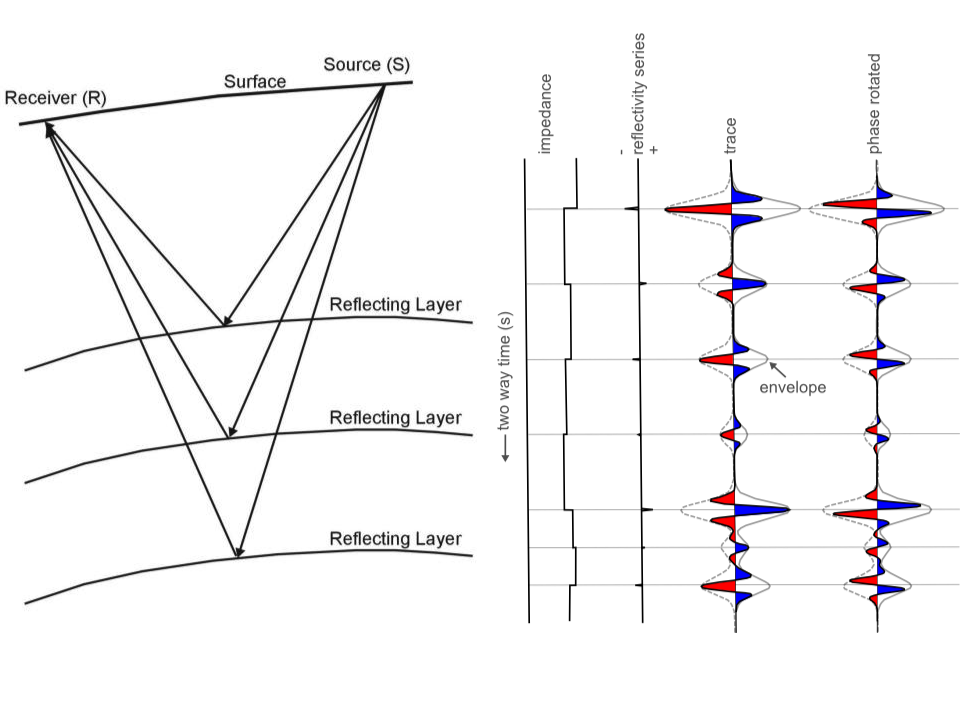
\includegraphics[scale=0.4]{figures/seismic_reflection_principal.png}
\caption{Reflection Seismology \cite{seisreflectionepa} \cite{seisreflectionagile}}
\label{seismic_reflection}
\end{figure}

%A landscape figure should be shown below. 
%%%%%%%%%%%%%%%%%%%%%%%%%%%%%%%%%%%%%%%%%%%%%%%%%%%%%%
%\begin{sidewaysfigure}[H]
%\centering
%\includegraphics[scale=.50]{figures/Penguins.jpg}
%\caption{TAMU figure - This is an example of a long figure title with a landscape figure.  Figure titles need to be single-spaced within and double spaced between in the list of figures.}
%\label{fig:tamu-fig1-1}
%\end{sidewaysfigure}
%%%%%%%%%%%%%%%%%%%%%%%%%%%%%%%%%%%%%%%%%%%%%%%%%%%%%%

%\subsection{This is a Very Long Subsection Title This is a Very Long Subsection Title}


\section{Motivations}

\subsection{Big Data and Scalability}

The emerging challenges in petroleum domain are the burst increase of the volume size of acquired data and high-speed streaming data from sensors in wells that need to be analyzed on time. Many types of captured data are used to create models and images of the Earth's structure and layers 5,000-35,000 feet below the surface and to describe activities around the wells themselves, such as machinery performance, oil flow rates and pressures. With approximately one million wells currently producing oil and/or gas in the United States alone, and many more gauges monitoring performance, this dataset is growing daily \cite{bigdataofindustry}. Moreover, not only the real world datasets, but also the dimensions and complexity of datasets themselves increase dramatically, such as 4D even 5D and high density seismic data. The traditional HPC solutions are able to improve the performance of many computation-intensive models, however,  most processing models are also data-intensive which are still the bottleneck for the whole workflow. 

In many the data- and technology-driven industries, big data analytics platforms and cloud computing technologies have made great progress in recent years toward meeting the requirements of exploring the valuable information from fast-growing data volumes and varieties.  Hadoop and Spark are currently the most popular open source big data platforms that provide scalable solutions to store and process big data, which deliver dynamic, elastic and scalable data storage and analytics solutions to tackle the challenges in the big data era. These platforms allow data scientists to explore massive datasets and extract valuable information with scalable performance. Many technologies advances in statistics, machine learning, NoSQL database, and in-memory computing from both industry and academia continue to stimulate new innovations in the data analytics field.

\subsection{Complicated Workflow}
Since the seismic data processing flow involves deep knowledges of geophysics, data science and computer science, it requests intensive collaborations among the scientists and developers from many different fields. This situation has long been another bottleneck for the whole system. For an instance, most scientists are using MATLAB code to build their models, which is usually hard to translate to MPI codes. In most cases, the program needs to be reconstructed and parallelized by software engineers. For this situation, it is already a big challenge to both geoscientist and software engineers to understand each other's work, not to mention to maintenance or optimize the huge amount of legacy code in this industry.


\section{Objectives}

Geophysicists need an ease-to-use and scalable platform that allows them to advance the seismic data exploration process, design more intelligent algorithms to increase the drilling success rate. By Incorporating the latest big data analytics technology with the geoscience domain knowledge will speed up their innovations in the exploration/interpretation phase.

Although there are some big data analytics platforms available in the market, they are not widely deployed in the petroleum industry since there is a big gap between these platforms and the special needs of the industry. For example, the seismic data formats are not supported by any of these platforms, and the machine learning algorithms need to be integrated with geology and geophysics knowledge to make the findings meaningful.

The objectives of the work are to develop a seismic data analytics software development kits (SDK) to enable geophysicists to easily leverage the latest big data analytics technology to improve the seismic data exploration.




